\documentclass{article}

\usepackage{amsmath,amssymb,geometry,tikz}
\usepackage{xepersian}

\setlength{\parindent}{0pt}
\setlength{\parskip}{3mm}

\newcounter{questionnumber}
\setcounter{questionnumber}{1}

\newcommand{\Q}{
\textbf{سوال \thequestionnumber)}
\stepcounter{questionnumber}
}

\newcommand{\eqn}[1]{
\begin{equation}\begin{split}
#1
\end{split}\end{equation}
}

\begin{document}
\LARGE
\begin{center}
\settextfont{IranNastaliq}

به نام زیبایی

%\begin{figure}[h]
%\centering
%\includegraphics[width=30mm]{kntu_logo.eps}
%\end{figure}

تمرینات سری پنجم درس احتمال مهندسی

\end{center}
\hrulefill
\large

\Q

نقطه‌ای را از داخل مربع به تصادف انتخاب می‌کنیم. احتمال آنکه فاصله‌ی این نقطه تا مرکز مربع، از فاصله‌ی این نقطه تا هر یک از رئوس مربع بیشتر باشد چقدر است؟

\Q

الف) در یک صفحه‌ی شطرنجی 8 در 8، یک مهره‌ی رخ سفید به تصادف در یکی از خانه‌های این صفحه قرار می‌گیرد. سپس، یک مهره‌ی رخ سیاه را به تصادف در یکی از خانه‌های این صفحه قرار می‌دهیم. با چه احتمالی، رخ سیاه در معرض حمله‌ی رخ سفید قرار می‌گیرد؟ (حرکت رخ، به صورت افقی یا عمودی در صفحه است)

ب) یک مهره‌ی شاه سفید، در یکی از گوشه‌های یک صفحه‌ی شطرنجی 8 در 8 قرار دارد. دو رخ سیاه به تصادف در دو خانه‌ی این صفحه قرار می‌گیرند. با چه احتمالی، شاه سفید مات می‌شود؟ (مات شدن شاه، زمانی اتفاق می‌افتد که نوبت حرکت شاه بوده و با هر حرکت، در معرض حمله‌ی یکی از مهره‌های دشمن قرار گیرد)

\begin{figure}[h]
\centering
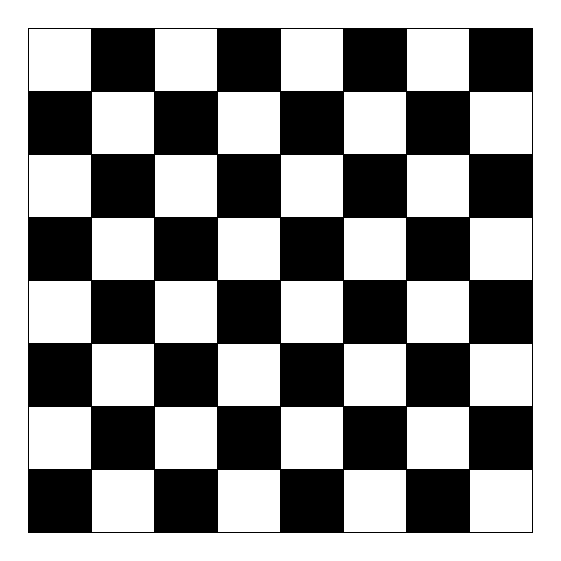
\begin{tikzpicture}
\filldraw[fill=black](-3.2,-3.2)--(-2.4000000000000004,-3.2)--(-2.4000000000000004,-2.4000000000000004)--(-3.2,-2.4000000000000004)--(-3.2,-3.2);
\filldraw[fill=white](-3.2,-2.4000000000000004)--(-2.4000000000000004,-2.4000000000000004)--(-2.4000000000000004,-1.6000000000000003)--(-3.2,-1.6000000000000003)--(-3.2,-2.4000000000000004);
\filldraw[fill=black](-3.2,-1.6)--(-2.4000000000000004,-1.6)--(-2.4000000000000004,-0.8)--(-3.2,-0.8)--(-3.2,-1.6);
\filldraw[fill=white](-3.2,-0.8)--(-2.4000000000000004,-0.8)--(-2.4000000000000004,0.0)--(-3.2,0.0)--(-3.2,-0.8);
\filldraw[fill=black](-3.2,0.0)--(-2.4000000000000004,0.0)--(-2.4000000000000004,0.8)--(-3.2,0.8)--(-3.2,0.0);
\filldraw[fill=white](-3.2,0.8)--(-2.4000000000000004,0.8)--(-2.4000000000000004,1.6)--(-3.2,1.6)--(-3.2,0.8);
\filldraw[fill=black](-3.2,1.6)--(-2.4000000000000004,1.6)--(-2.4000000000000004,2.4000000000000004)--(-3.2,2.4000000000000004)--(-3.2,1.6);
\filldraw[fill=white](-3.2,2.4000000000000004)--(-2.4000000000000004,2.4000000000000004)--(-2.4000000000000004,3.2)--(-3.2,3.2)--(-3.2,2.4000000000000004);
\filldraw[fill=white](-2.4000000000000004,-3.2)--(-1.6000000000000003,-3.2)--(-1.6000000000000003,-2.4000000000000004)--(-2.4000000000000004,-2.4000000000000004)--(-2.4000000000000004,-3.2);
\filldraw[fill=black](-2.4000000000000004,-2.4000000000000004)--(-1.6000000000000003,-2.4000000000000004)--(-1.6000000000000003,-1.6000000000000003)--(-2.4000000000000004,-1.6000000000000003)--(-2.4000000000000004,-2.4000000000000004);
\filldraw[fill=white](-2.4000000000000004,-1.6)--(-1.6000000000000003,-1.6)--(-1.6000000000000003,-0.8)--(-2.4000000000000004,-0.8)--(-2.4000000000000004,-1.6);
\filldraw[fill=black](-2.4000000000000004,-0.8)--(-1.6000000000000003,-0.8)--(-1.6000000000000003,0.0)--(-2.4000000000000004,0.0)--(-2.4000000000000004,-0.8);
\filldraw[fill=white](-2.4000000000000004,0.0)--(-1.6000000000000003,0.0)--(-1.6000000000000003,0.8)--(-2.4000000000000004,0.8)--(-2.4000000000000004,0.0);
\filldraw[fill=black](-2.4000000000000004,0.8)--(-1.6000000000000003,0.8)--(-1.6000000000000003,1.6)--(-2.4000000000000004,1.6)--(-2.4000000000000004,0.8);
\filldraw[fill=white](-2.4000000000000004,1.6)--(-1.6000000000000003,1.6)--(-1.6000000000000003,2.4000000000000004)--(-2.4000000000000004,2.4000000000000004)--(-2.4000000000000004,1.6);
\filldraw[fill=black](-2.4000000000000004,2.4000000000000004)--(-1.6000000000000003,2.4000000000000004)--(-1.6000000000000003,3.2)--(-2.4000000000000004,3.2)--(-2.4000000000000004,2.4000000000000004);
\filldraw[fill=black](-1.6,-3.2)--(-0.8,-3.2)--(-0.8,-2.4000000000000004)--(-1.6,-2.4000000000000004)--(-1.6,-3.2);
\filldraw[fill=white](-1.6,-2.4000000000000004)--(-0.8,-2.4000000000000004)--(-0.8,-1.6000000000000003)--(-1.6,-1.6000000000000003)--(-1.6,-2.4000000000000004);
\filldraw[fill=black](-1.6,-1.6)--(-0.8,-1.6)--(-0.8,-0.8)--(-1.6,-0.8)--(-1.6,-1.6);
\filldraw[fill=white](-1.6,-0.8)--(-0.8,-0.8)--(-0.8,0.0)--(-1.6,0.0)--(-1.6,-0.8);
\filldraw[fill=black](-1.6,0.0)--(-0.8,0.0)--(-0.8,0.8)--(-1.6,0.8)--(-1.6,0.0);
\filldraw[fill=white](-1.6,0.8)--(-0.8,0.8)--(-0.8,1.6)--(-1.6,1.6)--(-1.6,0.8);
\filldraw[fill=black](-1.6,1.6)--(-0.8,1.6)--(-0.8,2.4000000000000004)--(-1.6,2.4000000000000004)--(-1.6,1.6);
\filldraw[fill=white](-1.6,2.4000000000000004)--(-0.8,2.4000000000000004)--(-0.8,3.2)--(-1.6,3.2)--(-1.6,2.4000000000000004);
\filldraw[fill=white](-0.8,-3.2)--(0.0,-3.2)--(0.0,-2.4000000000000004)--(-0.8,-2.4000000000000004)--(-0.8,-3.2);
\filldraw[fill=black](-0.8,-2.4000000000000004)--(0.0,-2.4000000000000004)--(0.0,-1.6000000000000003)--(-0.8,-1.6000000000000003)--(-0.8,-2.4000000000000004);
\filldraw[fill=white](-0.8,-1.6)--(0.0,-1.6)--(0.0,-0.8)--(-0.8,-0.8)--(-0.8,-1.6);
\filldraw[fill=black](-0.8,-0.8)--(0.0,-0.8)--(0.0,0.0)--(-0.8,0.0)--(-0.8,-0.8);
\filldraw[fill=white](-0.8,0.0)--(0.0,0.0)--(0.0,0.8)--(-0.8,0.8)--(-0.8,0.0);
\filldraw[fill=black](-0.8,0.8)--(0.0,0.8)--(0.0,1.6)--(-0.8,1.6)--(-0.8,0.8);
\filldraw[fill=white](-0.8,1.6)--(0.0,1.6)--(0.0,2.4000000000000004)--(-0.8,2.4000000000000004)--(-0.8,1.6);
\filldraw[fill=black](-0.8,2.4000000000000004)--(0.0,2.4000000000000004)--(0.0,3.2)--(-0.8,3.2)--(-0.8,2.4000000000000004);
\filldraw[fill=black](0.0,-3.2)--(0.8,-3.2)--(0.8,-2.4000000000000004)--(0.0,-2.4000000000000004)--(0.0,-3.2);
\filldraw[fill=white](0.0,-2.4000000000000004)--(0.8,-2.4000000000000004)--(0.8,-1.6000000000000003)--(0.0,-1.6000000000000003)--(0.0,-2.4000000000000004);
\filldraw[fill=black](0.0,-1.6)--(0.8,-1.6)--(0.8,-0.8)--(0.0,-0.8)--(0.0,-1.6);
\filldraw[fill=white](0.0,-0.8)--(0.8,-0.8)--(0.8,0.0)--(0.0,0.0)--(0.0,-0.8);
\filldraw[fill=black](0.0,0.0)--(0.8,0.0)--(0.8,0.8)--(0.0,0.8)--(0.0,0.0);
\filldraw[fill=white](0.0,0.8)--(0.8,0.8)--(0.8,1.6)--(0.0,1.6)--(0.0,0.8);
\filldraw[fill=black](0.0,1.6)--(0.8,1.6)--(0.8,2.4000000000000004)--(0.0,2.4000000000000004)--(0.0,1.6);
\filldraw[fill=white](0.0,2.4000000000000004)--(0.8,2.4000000000000004)--(0.8,3.2)--(0.0,3.2)--(0.0,2.4000000000000004);
\filldraw[fill=white](0.8,-3.2)--(1.6,-3.2)--(1.6,-2.4000000000000004)--(0.8,-2.4000000000000004)--(0.8,-3.2);
\filldraw[fill=black](0.8,-2.4000000000000004)--(1.6,-2.4000000000000004)--(1.6,-1.6000000000000003)--(0.8,-1.6000000000000003)--(0.8,-2.4000000000000004);
\filldraw[fill=white](0.8,-1.6)--(1.6,-1.6)--(1.6,-0.8)--(0.8,-0.8)--(0.8,-1.6);
\filldraw[fill=black](0.8,-0.8)--(1.6,-0.8)--(1.6,0.0)--(0.8,0.0)--(0.8,-0.8);
\filldraw[fill=white](0.8,0.0)--(1.6,0.0)--(1.6,0.8)--(0.8,0.8)--(0.8,0.0);
\filldraw[fill=black](0.8,0.8)--(1.6,0.8)--(1.6,1.6)--(0.8,1.6)--(0.8,0.8);
\filldraw[fill=white](0.8,1.6)--(1.6,1.6)--(1.6,2.4000000000000004)--(0.8,2.4000000000000004)--(0.8,1.6);
\filldraw[fill=black](0.8,2.4000000000000004)--(1.6,2.4000000000000004)--(1.6,3.2)--(0.8,3.2)--(0.8,2.4000000000000004);
\filldraw[fill=black](1.6,-3.2)--(2.4000000000000004,-3.2)--(2.4000000000000004,-2.4000000000000004)--(1.6,-2.4000000000000004)--(1.6,-3.2);
\filldraw[fill=white](1.6,-2.4000000000000004)--(2.4000000000000004,-2.4000000000000004)--(2.4000000000000004,-1.6000000000000003)--(1.6,-1.6000000000000003)--(1.6,-2.4000000000000004);
\filldraw[fill=black](1.6,-1.6)--(2.4000000000000004,-1.6)--(2.4000000000000004,-0.8)--(1.6,-0.8)--(1.6,-1.6);
\filldraw[fill=white](1.6,-0.8)--(2.4000000000000004,-0.8)--(2.4000000000000004,0.0)--(1.6,0.0)--(1.6,-0.8);
\filldraw[fill=black](1.6,0.0)--(2.4000000000000004,0.0)--(2.4000000000000004,0.8)--(1.6,0.8)--(1.6,0.0);
\filldraw[fill=white](1.6,0.8)--(2.4000000000000004,0.8)--(2.4000000000000004,1.6)--(1.6,1.6)--(1.6,0.8);
\filldraw[fill=black](1.6,1.6)--(2.4000000000000004,1.6)--(2.4000000000000004,2.4000000000000004)--(1.6,2.4000000000000004)--(1.6,1.6);
\filldraw[fill=white](1.6,2.4000000000000004)--(2.4000000000000004,2.4000000000000004)--(2.4000000000000004,3.2)--(1.6,3.2)--(1.6,2.4000000000000004);
\filldraw[fill=white](2.4000000000000004,-3.2)--(3.2,-3.2)--(3.2,-2.4000000000000004)--(2.4000000000000004,-2.4000000000000004)--(2.4000000000000004,-3.2);
\filldraw[fill=black](2.4000000000000004,-2.4000000000000004)--(3.2,-2.4000000000000004)--(3.2,-1.6000000000000003)--(2.4000000000000004,-1.6000000000000003)--(2.4000000000000004,-2.4000000000000004);
\filldraw[fill=white](2.4000000000000004,-1.6)--(3.2,-1.6)--(3.2,-0.8)--(2.4000000000000004,-0.8)--(2.4000000000000004,-1.6);
\filldraw[fill=black](2.4000000000000004,-0.8)--(3.2,-0.8)--(3.2,0.0)--(2.4000000000000004,0.0)--(2.4000000000000004,-0.8);
\filldraw[fill=white](2.4000000000000004,0.0)--(3.2,0.0)--(3.2,0.8)--(2.4000000000000004,0.8)--(2.4000000000000004,0.0);
\filldraw[fill=black](2.4000000000000004,0.8)--(3.2,0.8)--(3.2,1.6)--(2.4000000000000004,1.6)--(2.4000000000000004,0.8);
\filldraw[fill=white](2.4000000000000004,1.6)--(3.2,1.6)--(3.2,2.4000000000000004)--(2.4000000000000004,2.4000000000000004)--(2.4000000000000004,1.6);
\filldraw[fill=black](2.4000000000000004,2.4000000000000004)--(3.2,2.4000000000000004)--(3.2,3.2)--(2.4000000000000004,3.2)--(2.4000000000000004,2.4000000000000004);
\end{tikzpicture}
\end{figure}

\Q

از مجموعه‌ی زیرمجموعه‌های مجموعه‌ی
$
\{1,2,3,\cdots,n\}
$
، دو زیرمجموعه‌‌‌ی متمایز به تصادف انتخاب می‌کنیم. با چه احتمالی، این دو زیرمجموعه ناسازگارند؟

\end{document}